\section[Intro]{Introduzione}
    \begin{frame}
        \frametitle{Contenuti}
        \transblindsvertical
        \tableofcontents[currentsection]
    \end{frame}

\setbeamercolor{background canvas}{use=structure,bg=white}
\setbeamercolor{background}{use=structure,bg=white}

    \begin{frame}{Il sistema solare}
        \begin{block}{Descrizione fisica}
            N corpi di massa $m_i$ che interagiscono secondo la legge di gravitazione universale $\Rightarrow$ N equazioni differenziali del secondo ordine accoppiate
            \\
            \begin{equation}
                \vec{a_i} = -\sum_{i\neq j}\frac{Gm_j}{r_{ij}^2}\frac{\vec r_{ij}}{r_{ij}}\,\,\,\,\,\,\,\,\forall i=1,\dots N
            \end{equation}
        \end{block}
    
        \begin{figure}
            \centering
            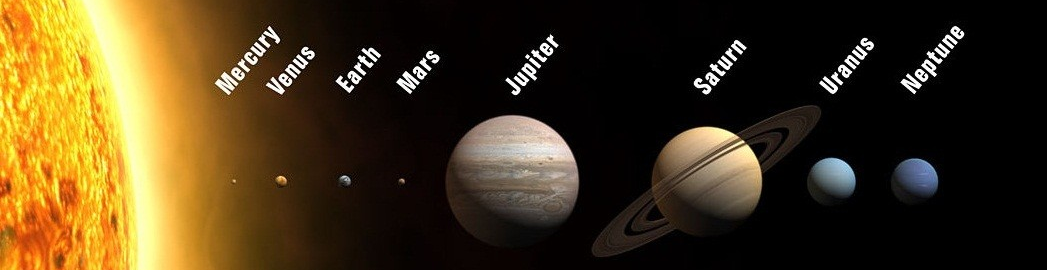
\includegraphics[width=\textwidth]{1_intro/siss.png}
            %\caption{Caption}
            %\label{fig:enter-label}
        \end{figure}       
    \end{frame}

    \begin{frame}{Il progetto}
        \begin{block}{Valutazione della coerenza della simulazione}
            \begin{enumerate}
                \item Studio delle quantità "conservate":
                \begin{itemize}
                    \item Energia totale
                    \item Momento angolare totale
                    \item eccentricità dell'orbita
                    \item distanza dal sole
                    \item inclinazione dell'orbita
                \end{itemize}
                \item Studio della dipendenza dai parametri:
                \begin{itemize}
                    \item Posizione e velocità dei corpi
                    \item Tempo di simulazione
                    \item Granularità
                    \item Metodo di approssimazione
                \end{itemize}              
            \end{enumerate}
        \end{block}

        \begin{block}{Efficienza}
            \begin{enumerate}
                \item Confronto tra C++ e Python
                \item Utilizzo dei due linguaggi per scopi differenti
            \end{enumerate}
        \end{block}
        
    \end{frame}
